% data_pipeline_tikz.tex  --  data processing flow for the Tenet/foreign-influence
% podcast project. Standalone-compilable (pdflatex). Drop the tikzpicture into the
% paper, or compile as-is for a figure. PI: Jared Edgerton (PSU).
\documentclass[border=8pt]{standalone}
\usepackage{tikz}
\usetikzlibrary{arrows.meta, positioning, fit, backgrounds, calc}
\begin{document}
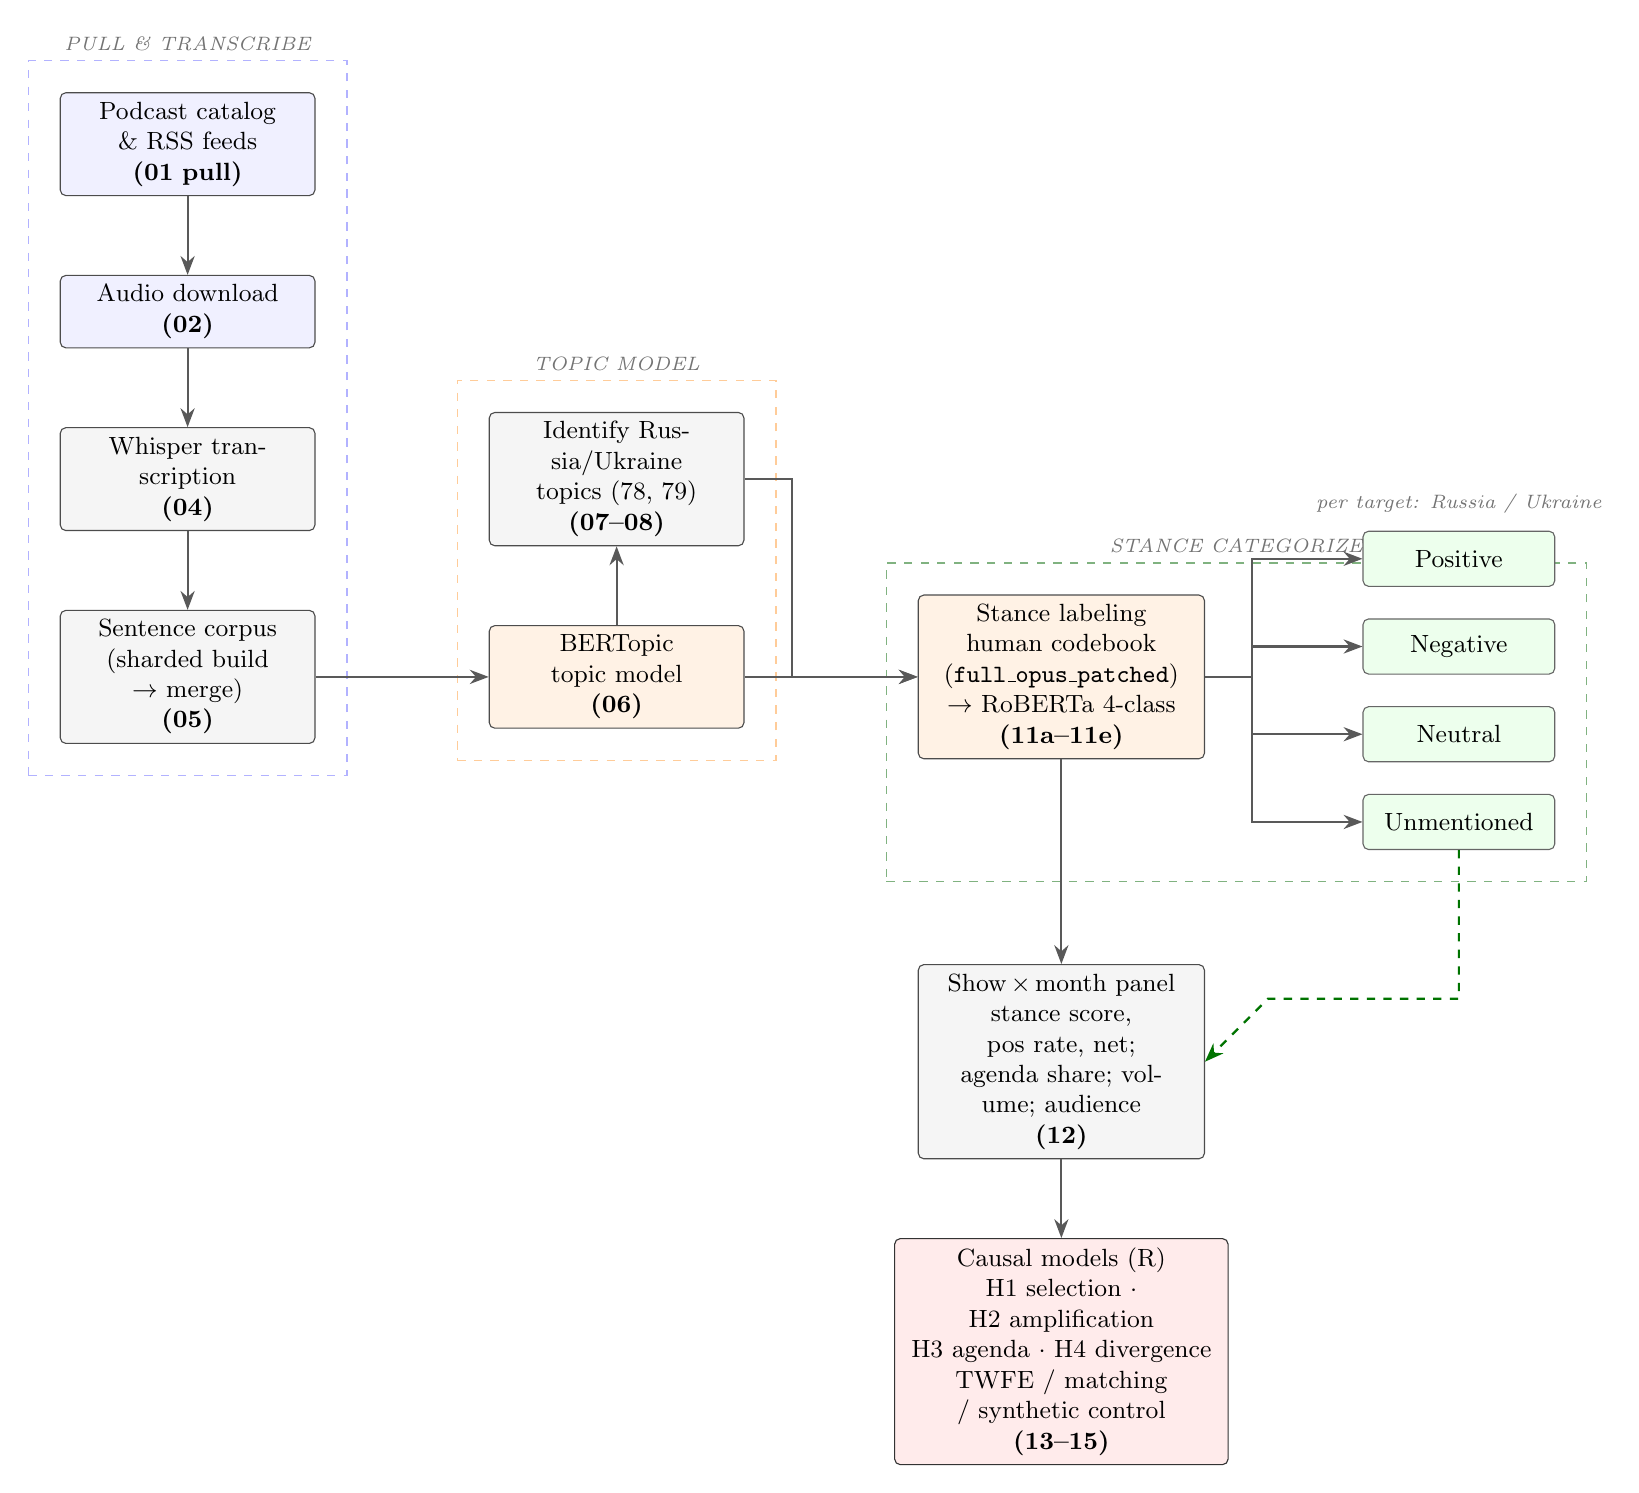
\begin{tikzpicture}[
  font=\small,
  node distance=10mm and 14mm,
  >={Stealth[length=2.4mm]},
  pull/.style   ={rectangle, rounded corners=2pt, draw=black!70, fill=blue!6,   text width=30mm, align=center, minimum height=9mm},
  proc/.style   ={rectangle, rounded corners=2pt, draw=black!70, fill=gray!8,   text width=30mm, align=center, minimum height=9mm},
  model/.style  ={rectangle, rounded corners=2pt, draw=black!70, fill=orange!10,text width=30mm, align=center, minimum height=9mm},
  cat/.style    ={rectangle, rounded corners=2pt, draw=black!60, fill=green!7,  text width=22mm, align=center, minimum height=7mm},
  analy/.style  ={rectangle, rounded corners=2pt, draw=black!80, fill=red!8,    text width=30mm, align=center, minimum height=9mm},
  stagelbl/.style   ={font=\scriptsize\itshape, text=black!55},
  arr/.style    ={->, thick, draw=black!65}
]

% ---- PULL / PROCESS column (left, top-to-bottom) ----
\node[pull]  (rss)   {Podcast catalog \& RSS feeds\\\textbf{(01 pull)}};
\node[pull]  (audio) [below=of rss]   {Audio download\\\textbf{(02)}};
\node[proc]  (asr)   [below=of audio] {Whisper transcription\\\textbf{(04)}};
\node[proc]  (corp)  [below=of asr]   {Sentence corpus\\(sharded build $\to$ merge)\\\textbf{(05)}};

% ---- TOPIC column (middle) ----
\node[model] (bert)  [right=22mm of corp] {BERTopic topic model\\\textbf{(06)}};
\node[proc]  (rid)   [above=of bert] {Identify Russia/Ukraine\\topics (78, 79)\\\textbf{(07--08)}};

% ---- LABELING column ----
\node[model] (label) [right=22mm of bert, text width=34mm]
   {Stance labeling\\ human codebook (\texttt{full\_opus\_patched})\\ $\to$ RoBERTa 4-class\\\textbf{(11a--11e)}};

% ---- CATEGORIES (the 4 stance classes, per target) ----
\node[cat] (pos) [right=20mm of label, yshift=15mm] {Positive};
\node[cat] (neg) [below=4mm of pos] {Negative};
\node[cat] (neu) [below=4mm of neg] {Neutral};
\node[cat] (unm) [below=4mm of neu] {Unmentioned};
\node[stagelbl, above=1mm of pos] {per target: Russia / Ukraine};

% ---- PANEL + ANALYSIS ----
\node[proc]  (panel) [below=26mm of label, text width=34mm]
   {Show\,$\times$\,month panel\\ stance score, pos rate, net;\\ agenda share; volume; audience\\\textbf{(12)}};
\node[analy] (anal)  [below=of panel, text width=40mm]
   {Causal models (R)\\ H1 selection $\cdot$ H2 amplification\\ H3 agenda $\cdot$ H4 divergence\\ TWFE / matching / synthetic control\\\textbf{(13--15)}};

% ---- edges ----
\draw[arr] (rss)   -- (audio);
\draw[arr] (audio) -- (asr);
\draw[arr] (asr)   -- (corp);
\draw[arr] (corp)  -- (bert);
\draw[arr] (bert)  -- (rid);
\draw[arr] (rid.east) -- ++(6mm,0) |- (label.west);
\draw[arr] (bert)  -- (label);
\draw[arr] (label.east) -- ++(6mm,0) |- (pos.west);
\draw[arr] (label.east) -- ++(6mm,0) |- (neg.west);
\draw[arr] (label.east) -- ++(6mm,0) |- (neu.west);
\draw[arr] (label.east) -- ++(6mm,0) |- (unm.west);
\draw[arr] (label) -- (panel);
\draw[arr] (panel) -- (anal);
% categories feed the panel
\draw[arr, dashed, draw=green!45!black] (unm.south) |- ($(panel.east)+(8mm,8mm)$) -- (panel.east);

% ---- stage banners ----
\begin{scope}[on background layer]
  \node[fit=(rss)(corp), draw=blue!30, dashed, inner sep=4mm, label={[stagelbl]above:PULL \& TRANSCRIBE}] {};
  \node[fit=(rid)(bert), draw=orange!40, dashed, inner sep=4mm, label={[stagelbl]above:TOPIC MODEL}] {};
  \node[fit=(label)(unm), draw=green!40!black!50, dashed, inner sep=4mm, label={[stagelbl]above:STANCE CATEGORIZE}] {};
\end{scope}

\end{tikzpicture}
\end{document}
